\chapter{The group structure of the cube}
A 3 by 3 by 3 cube has 6 fundamental moves. (Write out what they are.)
Claim that Rubik's cube in Figure~\ref{fig:solved-cube} under its fundamental moves can be view as a group, in more details, a permutation group.
\begin{figure}[h]
    \centering
    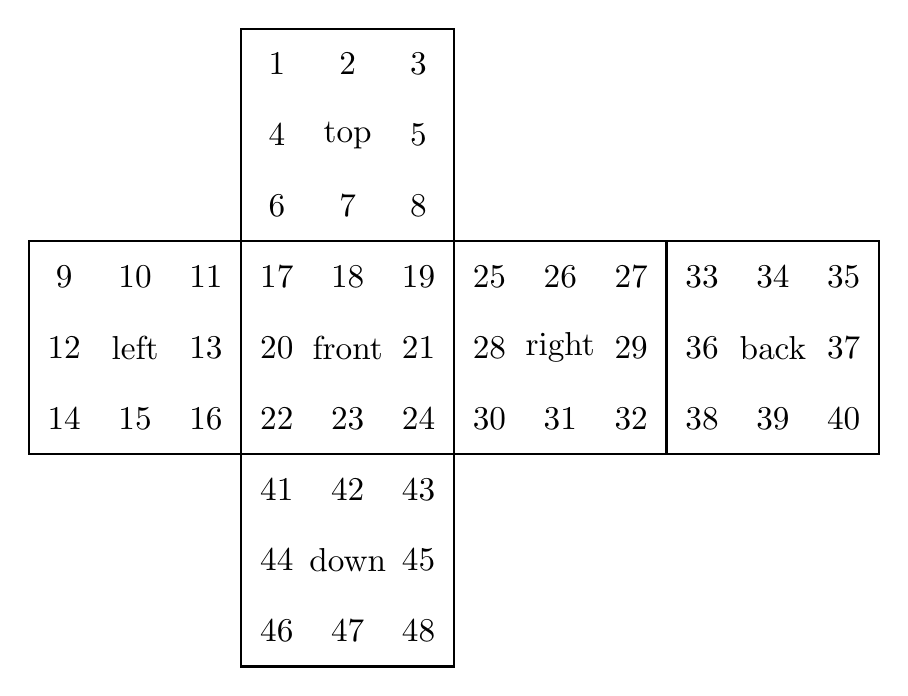
\begin{tikzpicture}[scale=0.9]
        % Draw the outlines.
        \draw[thick] (4.5,-0.5) -- (7.5,-0.5) -- (7.5,-9.5) -- (4.5,-9.5) -- cycle;
        \draw[thick] (1.5,-3.5) -- (13.5,-3.5) -- (13.5,-6.5) -- (1.5,-6.5) -- cycle;
        \draw[thick] (10.5,-3.5) -- (10.5,-6.5);
        % Specify the top face.
        \node[thick, scale=1.2] at (5,-1) {1};
        \node[thick, scale=1.2] at (6,-1) {2};
        \node[thick, scale=1.2] at (7,-1) {3};
        \node[thick, scale=1.2] at (5,-2) {4};
        \node[thick, scale=1.2] at (6,-2) {top};
        \node[thick, scale=1.2] at (7,-2) {5};
        \node[thick, scale=1.2] at (5,-3) {6};
        \node[thick, scale=1.2] at (6,-3) {7};
        \node[thick, scale=1.2] at (7,-3) {8};
        % Specify the left face.
        \node[thick, scale=1.2] at (2,-4) {9};
        \node[thick, scale=1.2] at (3,-4) {10};
        \node[thick, scale=1.2] at (4,-4) {11};
        \node[thick, scale=1.2] at (2,-5) {12};
        \node[thick, scale=1.2] at (3,-5) {left};
        \node[thick, scale=1.2] at (4,-5) {13};
        \node[thick, scale=1.2] at (2,-6) {14};
        \node[thick, scale=1.2] at (3,-6) {15};
        \node[thick, scale=1.2] at (4,-6) {16};
        % Specify the front face.
        \node[thick, scale=1.2] at (5,-4) {17};
        \node[thick, scale=1.2] at (6,-4) {18};
        \node[thick, scale=1.2] at (7,-4) {19};
        \node[thick, scale=1.2] at (5,-5) {20};
        \node[thick, scale=1.2] at (6,-5) {front};
        \node[thick, scale=1.2] at (7,-5) {21};
        \node[thick, scale=1.2] at (5,-6) {22};
        \node[thick, scale=1.2] at (6,-6) {23};
        \node[thick, scale=1.2] at (7,-6) {24};
        % Specify the right face.
        \node[thick, scale=1.2] at (8,-4) {25};
        \node[thick, scale=1.2] at (9,-4) {26};
        \node[thick, scale=1.2] at (10,-4) {27};
        \node[thick, scale=1.2] at (8,-5) {28};
        \node[thick, scale=1.2] at (9,-5) {right};
        \node[thick, scale=1.2] at (10,-5) {29};
        \node[thick, scale=1.2] at (8,-6) {30};
        \node[thick, scale=1.2] at (9,-6) {31};
        \node[thick, scale=1.2] at (10,-6) {32};
        % Specify the rear face.
        \node[thick, scale=1.2] at (11,-4) {33};
        \node[thick, scale=1.2] at (12,-4) {34};
        \node[thick, scale=1.2] at (13,-4) {35};
        \node[thick, scale=1.2] at (11,-5) {36};
        \node[thick, scale=1.2] at (12,-5) {back};
        \node[thick, scale=1.2] at (13,-5) {37};
        \node[thick, scale=1.2] at (11,-6) {38};
        \node[thick, scale=1.2] at (12,-6) {39};
        \node[thick, scale=1.2] at (13,-6) {40};
        % Specify the down face.
        \node[thick, scale=1.2] at (5,-7) {41};
        \node[thick, scale=1.2] at (6,-7) {42};
        \node[thick, scale=1.2] at (7,-7) {43};
        \node[thick, scale=1.2] at (5,-8) {44};
        \node[thick, scale=1.2] at (6,-8) {down};
        \node[thick, scale=1.2] at (7,-8) {45};
        \node[thick, scale=1.2] at (5,-9) {46};
        \node[thick, scale=1.2] at (6,-9) {47};
        \node[thick, scale=1.2] at (7,-9) {48};
    \end{tikzpicture}
    \caption{Labeling of solved cube.}\label{fig:label-solved-cube}
\end{figure}
Since essentially, what each movement of Rubik's cube does is to send one cubie to another location. In order to illustrate this idea, we find a numbering system for it and we define the six fundamental moves as permutations.
